\pagestyle{empty} % Limpa o cabeçalho e o rodapé
\onehalfspacing % Espaçamento entre-linhas de 1,5
% \hyphenpenalty=10000 % To prevent hyphenation
\pretolerance=10000 % To avoif overful lines
%\selectlanguage{english}
\selectlanguage{brazilian}
\setcounter{ex}{0} % counter for exercises
%\pagenumbering{arabic} % Uncomment this line if you want renumber pages for each chapter
\renewcommand{\chaptername}{Tutorial}
\chapter{Homologia Dinâmica: \textit{Iterative pass}, dados lacunares e partições em POY}\label{tut11}
\rhead{\tiny Instituto de Biociências --USP: BIZ0433 - Inferência Filogenética: Filosofia, Método e Aplicações}
\cfoot{\tiny \cc \ccby \ccsa \href{http://creativecommons.org/licenses/by-sa/4.0/}{Creative Commons Attribution-ShareAlike 4.0 International License}}
%\vspace{5pt}
{\large \sc BIZ0433 - Inferência Filogenética: Filosofia, Método e Aplicações.}\par
%\vspace{10pt}
\par
\minitoc % for table of contents within the chapter
\newpage
\section*{}\addcontentsline{toc}{section}{Objetivo}
\onehalfspacing
\vspace*{5pt}
\begin{center}
\emph{\begin{large}Objetivo\end{large}}\label{tut11:Objetivo}
\vspace{2pt}
\end{center}
%% TEXTO DO RESUMO
O objetivo deste tutorial é introduzir o conceito de \textit{Iterative pass} em análises de homologia dinâmica e suas aplicações nos processos de refinamento de análises filogenéticas. Este tutorial também aborda, de forma breve, os efeitos de dados lacunares (\textit{missing data}) em análises filogenéticas e aponta para os cuidados que devem ser tomados ao analisar sequências nucleotídicas em POY para as regiões de \textit{gap} iniciais e finais. Finalmente, o tutorial introduz estratégias de particionamentos que visam (\textit{i}) minimizar efeitos indesejados de dados lacunares e (\textit{ii}) aumentar a eficiência computacional de POY durante análises filogenéticas.  Os arquivos associados a este tutorial estão disponíveis em \url{http://lhe.ib.usp.br/cladistica}. Você pode baixá-los diretamente com o seguinte comando:

\begin{center}
\small \texttt{wget http://lhe.ib.usp.br/downloads/tutorial\_11.zip}\\
\end{center}


\newpage
\pagestyle{fancy} % Inclui o cabeçalho definido no meta.tex
%\pagenumbering{arabic} % Números das páginas em arábicos
\begin{refsection}
\renewcommand*{\finalnamedelim}{\addspace\&\space} % Usar '&' ao invés de 'e'.
%
%% color base pairs
\newcommand{\A}{\textcolor{green}{\textbf{A}}}
\newcommand{\C}{\textcolor{blue}{\textbf{C}}}
\newcommand{\G}{\textcolor{gray}{\textbf{G}}}
\newcommand{\T}{\textcolor{red}{\textbf{T}}}
\newcommand{\gap}{\textcolor{black}{\textbf{-}}}


%%%%%%%%%%%%%%%%%%%%%%%%%%%% HERE TEXT STARTS %%%%%%%%%%%%%%%%%%%%%%%%%%%%
\section{Iterative Pass}\label{tut11:ip}
	
Desde que o conceito de \textit{alinhamento} (ou \textit{alinhamento múltiplo}) foi apresentado (Tutorial \ref{tut8}), ficou evidente não só sua importância em inferência filogenética, bem como o quão dependente alinhamentos são de árvores-guia e os parâmetros numéricos de definem as funções de custo que norteiam a função objetiva do algoritmo (veja \textcite{Phillips_et_al_2000,Giribet_at_al_2002}). Embora definir o que é um ``bom alinhamento'' seja uma tarefa subjetiva e que alinhamentos ``reais'' provavelmente nunca serão encontrados na natureza, como argumenta \textcite{Wheeler_2012}, devemos considerar que o foco central em inferência filogenética é identificar a(s) melhor(es) topologia(as) de acordo com o critério de otimalidade que adotarmos. Consequentemente, os métodos que geram soluções melhores para este problema devem ser favorecidos \parencite[][]{Wheeler_and_Giribet_2009}.

A escolha da hipótese filogenética em inferência filogenética baseada em dados moleculares é feita pelo ordenamento do custo (distância patrística) de cada topologia em relação aos dados. No caso de sequências nucleotídicas sujeita a alinhamento, o cálculo deste custo define o que chamamos de \textit{Tree Alignment Problem} (\textbf{TAP}) -- \parencite[][]{Sankoff_1975}. Para resolver este problema, \textcite{Wheeler_1996} considerou o \textit{Tree Alignment Problem} como sendo um problema de otimização de caracteres em árvores filogenéticas dentro de um procedimento analítico chamado \textit{optimization alignment} ou \textit{direct optimization} (\textbf{OA/DO}). Este procedimento analítico é também conhecido como homologia dinâmica (senso \textcite{Wheeler_2001}), em contraste à forma tradicional de análises filogenéticas baseadas em dados moleculares na qual o alinhamento é um procedimento isolado que precede a busca por topologias ótimas, cujo resultado permite a obtenção de um alinhamento implícito (senso \textcite{Wheeler_2003a}).

Seja qual for o procedimento adotado para alinhamentos múltiplos, todos os programas examinados até o momento baseiam-se no algoritmo de Needleman-Wunsch \parencite{Needleman_and_Wunsch_1970,Phillips_et_al_2000}. Este algoritmo alinha pares de sequências independentemente do procedimento ser feito dentro do contexto de homologia estática para uma árvore-guia ou utilizando uma determinada topologia em homologia dinâmica por otimização direta. Em ambos os casos, estas são estratégias heurísticas que indiretamente (utilizando uma árvore-guia, no caso de homologias estáticas) ou diretamente (computando o custo de uma determinada topologia, no caso de homologia dinâmica) estimam as sequências para os nós de uma árvore filogenética. Esta estimativa nada mais é do que a atribuição dos estados de caráter aos ancestrais hipotéticos (\textbf{HTU}, de \textit{Hypothetical Taxonomic Units}), ou seja aos vértices da topologia.

Estimar sequências ancestrais \parencite[\textit{protosequences} senso][]{Sankoff_and_Cedergren_1973} que minimizam o custo de um alinhamento em uma topologia é atualmente um procedimento heurístico. Como vimos nos tutoriais anteriores, a otimização direta tende a encontrar soluções melhores em comparação com os procedimentos analíticos utilizando esquemas de homologia estática \parencite[veja Tutoriais \ref{tut9} e \ref{tut10}, ][]{Giribet_at_al_2002}. O caráter heurístico desse procedimento reside no fato de que o cálculo exato de um alinhamento múltiplo de \textit{n} sequências implicaria o mesmo número de dimensões de cálculo do algoritmo de Needleman-Wunsch. Teoricamente, a solução exata para esse problema multi-dimensional foi proposta por \textcite{Sankoff_et_al_1976} e já havia sido implementada para o alinhamento de três sequências por \textcite{Sankoff_and_Cedergren_1973} em uma versão tridimensional do algoritmo de \textcite{Needleman_and_Wunsch_1970}.

\textcite{Wheeler_2003b} concebeu um procedimento chamado \textit{iterative pass} (\textbf{IP}) que aplica otimização direta em três sequências, sejam elas hipotéticas ou não, simultaneamente. Este procedimento que também considera iterações analíticas que visam estabilizar o assinalamento de estados ancestrais aos vértices da topologia \parencite[\textit{i.e., iterative improvement}; veja][]{Wheeler_2003b} tende a gerar hipóteses filogenéticas ainda mais curtas que \textbf{DO}. No entanto o custo computacional deste algoritmo faz com que seu uso seja proibitivo durante a etapa de busca por topologias mais curtas (Figura \ref{tut11:fig:complexity}). Desta forma, historicamente seu uso está restrito a etapas de refinamento do alinhamento implícito no final da análise filogenética \parencite[\textit{e.g.},][]{Grant_et_al_2006,Dikow_2009,Jungfer_et_al_2013,Caira_et_al_2013,Pinto-da-Rocha_et_al_2014}. No entanto, \textcite{Machado_and_Marques_2013} revelaram outras propriedades do \textbf{IP} que transcendem apenas a redução em custos de topologias. Esses autores demonstram que esse algoritmo permite reduzir o número de topologias igualmente parcimoniosas e selecionar topologias que não seriam selecionadas com \textbf{DO}.

 %%%%%%%%%%%%%%%%%%%%%%%%%%% FIGURA TAP%%%%%%%%%%%%%%%%%%%%%%%%%%%
%  \vspace{-1em}
  \begin{figure}[H]
    %\ffigbox[\FBwidth]
       \centering
      {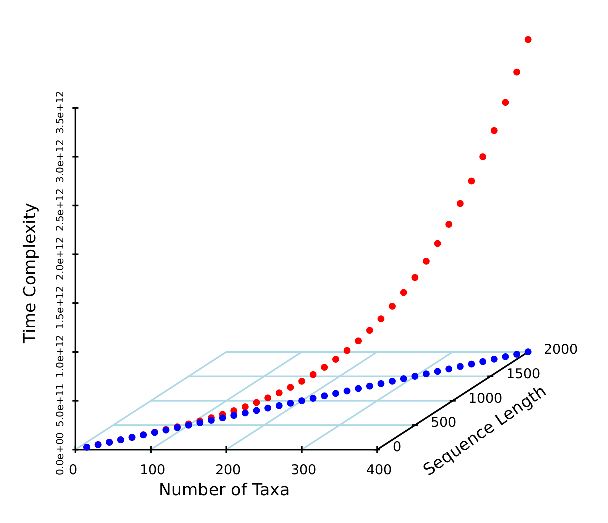
\includegraphics[scale=0.9]{figures/tut11/complexity.eps}}
	{\caption[Complexidade computacional de \textbf{DO} em comparação com \textbf{IP}.]{Complexidade computacional (medida em \textit{time complexity O}) de \textbf{DO} ($O(km^2)$) -- pontos azuis, onde $k$ é o número de terminais e $m$ o comprimento da sequência) em comparação com \textbf{IP} ($O(km^3)$) -- pontos laranjas -- em relação ao número de terminais e tamanho da sequência.}\label{tut11:fig:complexity}}
  \end{figure}

%%%%%%%%%%%%%%%%%%%%%%%%%%% FIM DA FIGURA TAP %%%%%%%%%%%%%%%%%%%%%


\subsection{Implementação}\label{tut11:ip:implementation}

A implementação de \textbf{IP} em POY é feita pelo argumento \texttt{iterative} do comando \texttt{set} do programa (veja seção 3.3.24 da documentação de POY) -- portanto, seria \texttt{set(iterative)}. Há duas formas de \textit{iterative pass} em POY. Por \textit{default}, POY computa a forma exata da otimização tridimensional, cujo comando literal seria: \texttt{set(iterative:exact)}. No comando \texttt{set(iterative:approximate)}, as iterações feitas durante a análise se aproximam do alinhamento tridimensional porém usando alinhamentos par a par. Este argumento não tem impacto drástico no tempo computacional e requer muito menos memória RAM durante a execução. No entanto, sua performance comparada com o cálculo exato de \textbf{IP} não está documentada na literatura. Seja como for, \textbf{IP} deve ser aplicado na fase final de refinamento de sua análise e os dados que tempos sobre as propriedade desse algoritmo estão baseadas na implementação exata.

\subsection{Tempo de execução}\label{tut11:ip:time}

Como pode ser visto na Figura \ref{tut11:fig:complexity}A--C to tempo computacional de \textit{iterative pass} incrementa consideravelmente quando comparado à otimização direta. A Figura \ref{tut11:fig:complexity2} ilustra com maiores detalhes esta relação. Observe que o incremento no número de terminais, quando o comprimento da sequência é fixo (100), ou o incremento no comprimento da sequência, quando o número de terminais é fixo (100), afetam de maneira distinta o tempo computacional (Figura \ref{tut11:fig:complexity2}A). O mesmo efeito é visto quando comparamos estas duas variáveis com os algoritmos de \textbf{DO} e \textbf{IP} (Figuras \ref{tut11:fig:complexity2}B e C).

 %%%%%%%%%%%%%%%%%%%%%%%%%%% FIGURA TAP%%%%%%%%%%%%%%%%%%%%%%%%%%%
%  \vspace{-1em}
  \begin{figure}[H]
    %\ffigbox[\FBwidth]
       \centering
      {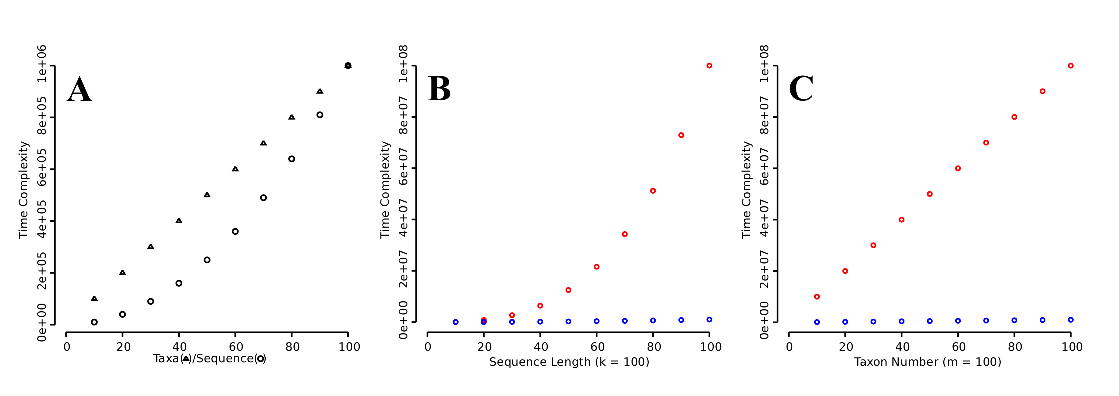
\includegraphics[scale=0.9]{figures/tut11/complexity_2.eps}}
	{\caption[Número de terminais, comprimento da sequência e complexidade computacional de \textbf{DO} em comparação com \textbf{IP}.]{Número de terminais, comprimento da sequência e complexidade computacional de \textbf{DO} em comparação com \textbf{IP}. \textbf{A} --  \textit{Time complexity $O$} vs. números de terminais (para $k=100$, triângulos) e comprimento de sequência (para $m=100$, circulos). \textbf{B} -- Comparação entre complexidade de \textbf{IP} (para $k=100$, circulos vermelhos) e \textbf{DO} (circulos azuis) vs. comprimento da sequência. \textbf{C} -- Comparação entre complexidade de \textbf{IP} (para $m=100$, circulos vermelhos) e \textbf{DO} (circulos azuis) vs. números de terminais.}\label{tut11:fig:complexity2}}
  \end{figure}

%%%%%%%%%%%%%%%%%%%%%%%%%%% FIM DA FIGURA TAP %%%%%%%%%%%%%%%%%%%%%

\stepcounter{ex}
\begin{blackBlock}{\textbf{Exercicio 11.\arabic{ex}}}\label{tut11:ex:11.1}

Considere o Script \ref{tut11:ip:script1}, abaixo, no qual a linha 3 configura o POY para fazer otimização por \textit{iterative pass} durante a busca utilizando 10 \textbf{RAS}+\textbf{SWAP} das sequências contidas em \texttt{partition2.fas} e reporte o tempo de execução, o custo e o número de topologias encontradas. Os arquivos \texttt{partition2\_6x30.fas}, \texttt{partition2\_6x60.fas} e \texttt{partition2\_6x100.fas} são modificações do arquivo \texttt{partition2.fas}. Todos contém 6 terminais apenas e diferem quanto ao tamanho das sequências (\textit{i.e.}, 30, 60 e 100, respectivamente). Neste exercício você deverá analizar esses dados utilizando \textbf{DO} e \textbf{IP} e o resultado de cada análise deverá ser colocado na Tabela \ref{tut11:table:ip:time:ex1}, abaixo.

\end{blackBlock}

\begin{lstlisting}[caption= Exemplo de \textit{script} para implementar \textit{iterative pass}.,label=tut11:ip:script1]
read("partition2.fas")
set(root:"Taxon1")
set(iterative:exact)
Build(10)
swap()
select()
report(timer:"Time to run IP",treestats)
exit()
\end{lstlisting}


%%%%%%%%%%%%%%%%%%%%%%%%%%% TABELA DE ANÁLISE IP (TEMPO) %%%%%%%%%%%%%%%%%%%%%%%%%%% 
%\begin{landscape}
\pagestyle{fancy}
\begin{center}

\begin{longtable}{|l|c|c|c|}
\caption[Tempo de execução em \textbf{IP}]{Efeito do comprimento das sequências durante a otimização por \textit{iterative pass}.} \label{tut11:table:ip:time:ex1} \\


\hline\hline \textbf{Dataset} & \textbf{Tempo (secs)}  & \textbf{Custo das MPTs\footnote{ topologias igualmente parcimoniosas (\textit{Most Parsimonious Trees})}} & \textbf{Número de MPTs} \\
\endfirsthead

\multicolumn{3}{c}{{\bfseries \tablename\ \thetable{} -- Continuação.}}\\
\hline\hline \textbf{Dataset} & \textbf{Tempo (secs)}  & \textbf{Custo das MPTs} & \textbf{Número de MPTs} \\
\endhead
%\hline \multicolumn{6}{r}{{--continua na próxima página}} \\ \hline
%\endfoot
\hline \hline
%\hline \multicolumn{6}{l}{Consulte a página \url{http://wiki.linuxquestions.org/wiki/Linux_software_equivalent_to_Windows_software}.}
\endlastfoot

\hline \texttt{partition2\_6x30.fas} &  & & \\
\hline \texttt{partition2\_6x60.fas} &  & & \\
\hline \texttt{partition2\_6x1000.fas} &  & & \\

\end{longtable}
\end{center}
%\end{landscape}
%%%%%%%%%%%%%%%%%%%%%%%%%%% FIM DA TABELA DE ANÁLISE IP (TEMPO) %%%%%%%%%%%%%%%%%%%%%%%%%%


\begin {myindentpar}{0.3cm}
\begin{enumerate}[\itshape i.]
	\item{Quais observações você pode fazer sobre essas análises?}

\begin{center}
\line(1,0){400}\\
\line(1,0){400}\\
\line(1,0){400}\\
\end{center}

\end{enumerate}
\end{myindentpar}

\subsection{Redução de MPTs}\label{tut11:ip:mpt}

Uma das propriedades pouco conhecidas de \textbf{IP} é que nem todas as árvores consideradas ótimas em \textbf{DO} possuem o mesmo custo quando submetidas ao refinamento. Essa propriedade foi documentada pela primeira vez por \textcite{Machado_and_Marques_2013} e sua utilidade é evidente: em análises por otimização direta que resultam em múltiplas topologias, o algoritmo de \textit{iterative pass} pode reduzir consideravelmente o número de topologias finais \parencite[veja também ][]{Caira_et_al_2013,Pinto-da-Rocha_et_al_2014}. O exercício a seguir demonstra essa propriedade.\\

\stepcounter{ex}
\begin{blackBlock}{\textbf{Exercicio 11.\arabic{ex}}}\label{tut11:ex:11.2}

Neste exercício você deverá executar dois \textit{scripts}. No primeiro, você deverá fazer uma análise utilizando \textbf{DO} e salvar as topologias encontradas. O segundo \textit{script} deverá fazer a rediagnose destas topologias via \textit{iterative pass}. As linhas de instrução destes \textit{scripts} devem obedecer as estruturas ilustradas abaixo.

\end{blackBlock}


Para o primeiro \textit{script},

\begin {myindentpar}{0.5cm}
\begin{enumerate}[\itshape 1.]

	\item{Leia o arquivo ''\texttt{partition2.fas}'',}
	\item{atribua a raíz ao  táxon ''\texttt{Taxon1}'',}
	\item{faça uma busca com o comando ''\texttt{search}'' por 10 minutos,}
	\item{selecione as topologias únicas e melhores,}
	\item{reporte no arquivo ''\texttt{collected\_trees.tre}'' as topologias encontradas e em ''\texttt{do.sts}'' os custos e o número de topologias encontradas,}
	\item{saia de POY.}

\end{enumerate}
\end{myindentpar}

Para o segundo \textit{script},

\begin {myindentpar}{0.5cm}
\begin{enumerate}[\itshape 1.]
	\item{Leia os arquivos ''\texttt{partition2.fas}'' e ''\texttt{collected\_trees.tre}'',}
	\item{atribua a raiz ao  taxon ''\texttt{Taxon1}'',}
	\item{implemente o algoritmo exato de IP,}
	\item{implemente o algoritmo de \textit{tree fusing} (\textit{default}) para as topologias contidas no arquivo ''\texttt{collected\_trees.tre}'',}
	\item{selecione as topologias únicas,}
	\item{reporte no arquivo ''\texttt{ip.sts}'' os custos e o número de topologias encontradas,}
	\item{saia de POY.}

\end{enumerate}
\end{myindentpar}

Finalmente, compare os conteúdos dos arquivos \texttt{do.sts} e \texttt{ip.sts} e faça um sumário dos seus resultados no espaço abaixo:

\begin{center}
\line(1,0){400}\\
\line(1,0){400}\\
\line(1,0){400}\\
\end{center}

\subsection{Outras propriedades de \textbf{IP}}\label{tut11:ip:other}

Há outras propriedades de \textbf{IP} documentadas por \textcite{Machado_and_Marques_2013} que devem ser ressaltadas. A primeira delas é que esse algoritmo quando conjugado com algoritmos de rearranjos se torna mais efetivo, principalmente \textit{tree--fusing} \parencite[][]{Goloboff_1999}. Em alguns casos \textbf{IP}+\textit{tree--fusing} é capaz de encontrar topologias que não estavam presentes no conjunto de topologias submetidas ao refinamento. No entanto, a propriedade mais interessante encontrada por esses autores está relacionada com a observação de que, para dados simulados no qual um conjunto de 10 topologias foram coletadas na fase de \textbf{DO} resultado de 10 iterações do comando \texttt{search}, \textbf{IP} considerou como topologia mais curta aquelas que foram consideradas subótimas por \textbf{DO} em 75\% das simulações! Isso se deve em parte às aproximações e ``\textit{short cuts}'' implementadas nos algoritmos de POY para reduzir o tempo computacional em \textbf{DO}. As implicações analíticas são óbvias. Sua análise será mais efetiva se você coletar um número razoável de topologias candidatas e submetê-las ao refinamento por \textbf{IP}+\textit{tree--fusing}. \textcite{Pinto-da-Rocha_et_al_2014}, por exemplo, reduziram o custo das topologias em até 3.3\% considerando topologias compiladas durante a análise de sensibilidade -- estratégia de busca conhecida como \textit{sensitivity search} \parencite[veja][]{Wheeler_et_al_2006}.\\


\stepcounter{ex}
\begin{blackBlock}{\textbf{Exercicio 11.\arabic{ex}}}\label{tut11:ex:11.3}

Neste exercício iremos explorar em conjunto a maioria dos conceitos apresentados neste e no tutorial anterior sobre análises por homologia dinâmica em POY. Este exercício lhe fornecerá as bases necessária para fazer uma boa análise de dados reais. O exercício é relativamente simples, mas requer atenção na confecção dos \textit{scripts} de execução para que você tenha bom controle do tempo de análise, bem como na coleção de informações que lhe permitirão responder às perguntas abaixo.

\end{blackBlock}

\begin {myindentpar}{0.3cm}
\begin{enumerate}[\itshape i.]

	\item{Qual é a diferença de custo entre a topologia encontrada por \textbf{DO} atribuindo pesos iguais para cada transformação e aquela encontrada por uma análise usando  \textit{sensitivity search} e diagnose por \textbf{IP}+\textit{tree--fusing}?}

	\item{A topologia final após \textit{sensitivity search} e \textbf{IP}+\textit{tree--fusing} é a mesma encontracas por \textbf{DO} sob os mesmos parâmetros de alinhamento?}

\end{enumerate}
\end{myindentpar}

	Para responder a essas perguntas você deverá fazer uma análise em POY utilizando os dados disponíveis nos arquivos \texttt{partition1.fas}, \texttt{partition2.fas} e \texttt{partition3.tnt}. Os resultados dessa sua análise deverão ser sumarizados no espaço abaixo:

\begin{center}
\line(1,0){400}\\
\line(1,0){400}\\
\line(1,0){400}\\
\end{center}

\section{Dados lacunares (\textit{missing data})}\label{tut11:missing}

Aqueles que já tiveram experiência com compilação e análise de dados reais em inferência filogenética devem ter se deparado com lacunas em suas matrizes de dados -- sejam elas genotípicas ou fenotípicas. Portanto, dados lacunares (\textit{missing data}) são muito comuns em matrizes reais. Para dados moleculares, em particular, principalmente quando o estudo envolve mais de uma região genômica (\textit{e.i.}, locus) e um número razoável de terminais, invariavelmente chega-se ao final da fase de compilação de dados com a dúvida se um determinado terminal deverá ou não ser incluído na análise em decorrência da observação de que para este há regiões -- ou caracteres -- que não foram obtidos. Há uma série de estudos que buscaram avaliar os efeitos de dados lacunares em inferência filogenética \parencite[veja][; e referências citadas]{Weins_1998,Weins_2003,Weins_2006,Weins_and_Morrill_2011,Grievink_et_al_2013}. No entanto, estes estudos são inconclusivos -- muito provavelmente resultado do caráter histórico e individual dos dados utilizados em inferência filogenética. A única generalização que se pode fazer é de que excesso de dados lacunares -- seja lá como ``excesso'' é definido -- tende a gerar múltiplas topologias igualmente parcimoniosas, pouco resolvidas e, para dados simulados, estimativas pouco acuradas de relacionamento filogenético \parencite{Weins_2003}. No entanto, a quantidade de dados lacunares de um terminal, por si só, não deve guiar decisões sobre sua exclusão ou não em análises filogenéticas \parencite{Weins_2003}. Isso porque, em alguns casos, a inserção destes terminais na análise pode melhorar drasticamente seu resultado final \parencite{Weins_2006}.

\subsection{Dados lacunares em POY}\label{tut11:missing:poy}

Embora alguns estudos empíricos e com dados simulados tenham avaliado o efeito de dados lacunares em inferência filogenética, estes se restringem a análises de homologia estática. Não há nenhuma avaliação sobre os efeitos de dados lacunares em homologia dinâmica que eu tenha conhecimento. No entanto, diante da situação na qual é necessário decidir se determinado terminal deve ou não ser incluído na análise devido a ausência de dados, aconselha-se a avaliar se os dados lacunares afetam ou não sua análise final. Isso pode ser feito avaliando o resultado da inferência filogenética incluindo ou não determinado(s) terminal(is) e/ou fragmento(s).

Ao contrário na maioria dos programas de inferência filogenética, POY não descarta uma base de dados após ler outra. Se um ``novo'' terminal não está presente no primeiro banco de dados, mas está presente no segundo, POY considerará que para este terminal inexiste dados para o primeiro fragmento, mas sem descartá-lo da análise. Por exemplo, considere dois bancos de dados:\\

\texttt{fasta\_1.fas}

\scriptsize
\texttt{taxon1~~~AAAA}

\texttt{taxon2~~~ACAA}

\texttt{taxon3~~~AAGA}

\texttt{taxon4~~~AAAT}

\normalsize

e

\texttt{fasta\_2.fas}

\scriptsize
\texttt{taxon1~~~CCCC}

\texttt{taxon3~~~CACC}

\texttt{taxon4~~~CCGC}

\texttt{taxon5~~~CCCT}

\normalsize

POY consideraria:

\scriptsize
\texttt{taxon1~~~AAAACCCC}

\texttt{taxon2~~~ACAA????}

\texttt{taxon3~~~AAGACACC}

\texttt{taxon4~~~AAATCCGC}

\texttt{taxon5~~~????CCCT}\\

\normalsize

Essa propriedade de POY tem um lado bom e um lado ruim. O lado bom é que o usuário não precisa se preocupar em manter bancos de dados distintos com os mesmos terminais. O lado ruim é que caso haja algum erro tipográfico em um terminal -- em um determinado banco de dados--, POY o considerará como outro terminal. Portanto, uma dica: usem nomes simples para os terminais e lembre-se que você poderá fazer substituições no final utilizando ferramentas como o \texttt{sed} ou até mesmo comandos internos de POY.

Há dois comandos em POY que estão estreitamente relacionados com a manipulação de dados lacunares. O primeiro deles é o o argumento \texttt{cross\_references} que pode ser implementado no comando \texttt{report()}. Seu uso permite gerar uma tabela indicando a distribuição de dados para os terminais. Considere o \textit{script} abaixo:\\

\begin{lstlisting}[caption= Exemplo de \textit{script} para implementar \texttt{cross\_references}.,label=tut11:missing:script1]
read("fasta1.fas","fasta2.fas")
report("refs.txt",cross_references)
exit()
\end{lstlisting}

O arquivo \texttt{refs.txt} teria o seguinte conteúdo:\\


\texttt{File~References:}

\texttt{Terminal~~~~fasta2.fas~~~~~~~~fasta1.fas}

\texttt{taxon1~~~~~~~~~~+~~~~~~~~~~~~~~~~~+}

\texttt{taxon2~~~~~~~~~~-~~~~~~~~~~~~~~~~~+}

\texttt{taxon3~~~~~~~~~~+~~~~~~~~~~~~~~~~~+}

\texttt{taxon4~~~~~~~~~~+~~~~~~~~~~~~~~~~~+}

\texttt{taxon5~~~~~~~~~~+~~~~~~~~~~~~~~~~~-}\\


onde \texttt{+} e \texttt{-} indicam presença e ausência, respectivamente, de determinado fragmento para um terminal.

O segundo comando é \texttt{select()}. Este comando permite selecionar subconjuntos de terminais, caracteres e topologias (veja seção 3.3.23 da documentação de POY). Por exemplo, o comando \texttt{select(terminals,files:("file.txt"))} ou simplesmente \texttt{select(files:("file.txt"))} seleciona o conteúdo do arquivo \texttt{file.txt} (\textit{i.e.}, terminais, caracteres ou topologias) para a análise. Esse comando, portanto, permitiria-lhe incluir e excluir terminais e caracteres para verificar o efeito de dados lacunares em sua análise.\\

\stepcounter{ex}
\begin{blackBlock}{\textbf{Exercicio 11.\arabic{ex}}}\label{tut11:ex:11.4}

Neste exercício você deverá fazer uma análise filogenética dos dados contido em \texttt{asteroids1.fas}, \texttt{asteroids2.fas} e \texttt{asteroids3.fas} que permita-lhe responder às perguntas abaixo.

\end{blackBlock}

\begin {myindentpar}{0.3cm}
\begin{enumerate}[\itshape i.]

	\item{Há dados lacunares nessas bases de dados? Quais?}

\begin{center}
\line(1,0){400}\\
\line(1,0){400}\\
\line(1,0){400}\\
\end{center}

	\item{A inclusão/exclusão de terminais para os quais há dados lacunares influencia as relações filogenéticas entre os terminais? Justifique.}

\begin{center}
\line(1,0){400}\\
\line(1,0){400}\\
\line(1,0){400}\\
\end{center}

\end{enumerate}
\end{myindentpar}

	\subsection{Dados lacunares em subpartições de POY}\label{tut11:missing:sub}

Há outras duas formas de dados lacunares que devem ser tratados adequadamente em POY. A primeira delas refere-se aos \textit{gaps} iniciais e finais inseridos na sequências em decorrência do sequenciamento diferencial da região de interesse. Estes \textit{gaps} não representam eventos de transformação putativas e devem ser removidos ou substituídos por \texttt{N}s. Também existe a possibilidade de que haja regiões em suas sequências onde exista falta de dados resultado do processo de sequenciamento. Nestes casos, é possível -- e de certa forma desejável -- criar subpartições em suas sequências. O objetivo destas partições é primariamente evitar artefatos analíticos. No entanto, há um outro motivo para a criação de subpartições e esta está relacionada com o desempenho de POY. Considere que quanto maior é o comprimento da sequência, maior é a dificuldade de encontrar soluções ótimas pelos algoritmos disponíveis. Afinal, o algoritmo de Needleman-Wunsch é míope. \textcite{Giribet_2001} notou que a criação de subpartições nos arquivos de dados pode reduzir drasticamente o tempo computacional das análises em POY. Subpartições podem ser criadas em BioEdit inserindo uma coluna de ``$\sim$s'' entre as regiões que você deseja particionar e posteriormente substituir esses ``$\sim$s'' por ``\texttt{{\#}}s'' em um editor de texto. Onde definir essas partições é arbitrário e o POY pode fazer isso automaticamente (veja o comando \texttt{auto\_sequence\_partition} na documentação de POY. Geralmente, essas partições são inseridas em regiões de alinhamento inequívoco que separam regiões sujeitas a alinhamento ou para as quais há dados lacunares.

O vídeo \texttt{partitions.avi} ilustra como isso deve ser feito. Este vídeo está no diretório associado a este tutorial ou pode ser visto no  \href{http://youtu.be/SeFRVRyBNbk}{YouTube}.\\


\section{Assignment 6}\label{tut11:assigment}

Neste trabalho você deverá apresentar uma reanálise de algum estudo filogenético já publicado de seu interesse que tenha sido feito com base em dados moleculares passíveis de análise por homologia dinâmica -- \textit{i.e.}, sujeitos a alinhamento. Ao selecionar o estudo de interesse, considere os recursos computacionais que possui a sua disposição, pois você já deve ter uma noção do custo computacional envolvido em análises por homologia dinâmica. 

\begin {myindentpar}{0.3cm}
\begin{enumerate}[\itshape a.]

 \item{\textbf{Forma de apresentação:}} Os resultados deste exercício deverão ser apresentados em um único documento em \textbf{formato PDF} contendo duas páginas:

    \begin {myindentpar}{0.3cm}
    \begin{enumerate}[\itshape 1.]
    \item{A primeira página deve apresentar um texto contendo três itens: \textit{i.} Introdução; \textit{ii.} métodos, e \textit{iii.} resultados e discussão.} 

	\begin {myindentpar}{0.3cm}
	\begin{enumerate}[\itshape i.]
		\item{\underline{Introdução}:} Neste item você deverá apresentar o trabalho que vocês escolheu abordar.\\
		\item{\underline{Métodos}:} Aqui você deverá fazer uma breve descrição dos métodos que você abordou, includino os comandos que definem a estratégia de busca utilizada.\\
		\item{\underline{Resultados e Discussão}:}  Finalmente, neste item você deverá fazer uma breve discussão sobre os resultados que você obteve em relação àqueles apresentados pelos autores.\\
	\end{enumerate}
	\end{myindentpar}

    \item{Na segunda página você deverá apresentar uma figura e \textbf{sua legenda} que sumarizem seus resultados. Esta figura será avaliada considerando a implementação de todos os recursos gráficos que foram apresentados ao londo do curso.}
    \end{enumerate}
    \end{myindentpar}


 \item{\textbf{Nome do arquivo:}} Os nomes do arquivo deverão obedecer o seguinte formato: \texttt{assignment\_06.pdf}.\\

 \item{\textbf{Data de entrega:}} Dia 06/06/2019 até as 14:00 hrs (antes da Aula 13).\\

 \item{\textbf{Forma de entrega:}} Fazer o \textit{upload} em \href{https://forms.gle/sf2Lq2VsRdkYU4Uf7}{https://forms.gle/sf2Lq2VsRdkYU4Uf7}.\\


\end{enumerate}
\end{myindentpar}



%%%%%%%%%%%%%%%%%%%%%%%%%%%% HERE ENDS TEXT AND ADDS REFERENCES %%%%%%%%%%%%%%%%%%%%%%%%%%%% 
\section{Referências}\label{tut11:refs}
\printbibliography[heading=none]
\end{refsection}
%  
